\documentclass{standalone}
\usepackage{tikz}
\usetikzlibrary{patterns, positioning}


\begin{document}
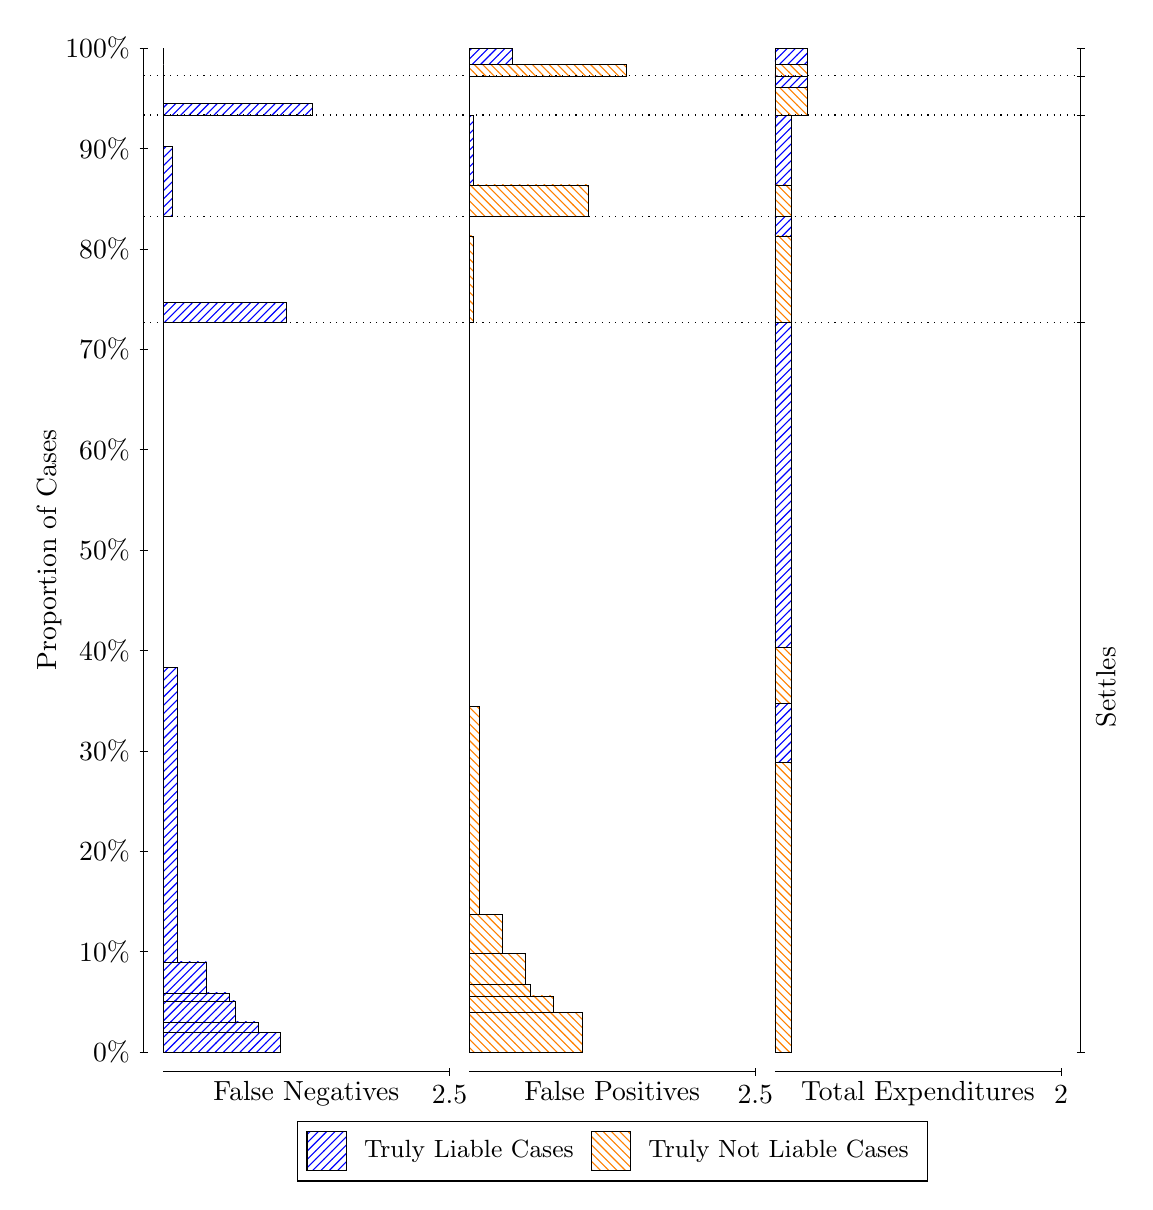
\begin{tikzpicture}
\draw[black, very thin] (1.5,1.75) -- (1.5,14.5);
\node[rotate=90, text=black, anchor=center] at (0.3, 8.125) {Proportion of Cases};
\draw[black, very thin] (1.45,1.75) -- (1.55,1.75);
\node[text=black, anchor=east] at (1.45, 1.75) {0\%};
\draw[black, very thin] (1.45,3.025) -- (1.55,3.025);
\node[text=black, anchor=east] at (1.45, 3.025) {10\%};
\draw[black, very thin] (1.45,4.3) -- (1.55,4.3);
\node[text=black, anchor=east] at (1.45, 4.3) {20\%};
\draw[black, very thin] (1.45,5.575) -- (1.55,5.575);
\node[text=black, anchor=east] at (1.45, 5.575) {30\%};
\draw[black, very thin] (1.45,6.85) -- (1.55,6.85);
\node[text=black, anchor=east] at (1.45, 6.85) {40\%};
\draw[black, very thin] (1.45,8.125) -- (1.55,8.125);
\node[text=black, anchor=east] at (1.45, 8.125) {50\%};
\draw[black, very thin] (1.45,9.4) -- (1.55,9.4);
\node[text=black, anchor=east] at (1.45, 9.4) {60\%};
\draw[black, very thin] (1.45,10.675) -- (1.55,10.675);
\node[text=black, anchor=east] at (1.45, 10.675) {70\%};
\draw[black, very thin] (1.45,11.95) -- (1.55,11.95);
\node[text=black, anchor=east] at (1.45, 11.95) {80\%};
\draw[black, very thin] (1.45,13.225) -- (1.55,13.225);
\node[text=black, anchor=east] at (1.45, 13.225) {90\%};
\draw[black, very thin] (1.45,14.5) -- (1.55,14.5);
\node[text=black, anchor=east] at (1.45, 14.5) {100\%};

\draw[black, very thin] (13.4,1.75) -- (13.4,14.5);
\draw[black, very thin] (13.35,1.75) -- (13.45,1.75);
\node[anchor=west] at (13.35, 1.75) {};
\draw[black, very thin] (13.35,11.019) -- (13.45,11.019);
\node[anchor=west] at (13.35, 11.019) {};
\draw[black, very thin] (13.35,12.365) -- (13.45,12.365);
\node[anchor=west] at (13.35, 12.365) {};
\draw[black, very thin] (13.35,13.649) -- (13.45,13.649);
\node[anchor=west] at (13.35, 13.649) {};
\draw[black, very thin] (13.35,14.146) -- (13.45,14.146);
\node[anchor=west] at (13.35, 14.146) {};
\draw[black, very thin] (13.35,14.5) -- (13.45,14.5);
\node[anchor=west] at (13.35, 14.5) {};

\draw[black, very thin, pattern color=blue, pattern=north east lines] (1.75,1.75) rectangle (3.2397,2.0016);
\draw[black, very thin, pattern color=blue, pattern=north east lines] (1.75,2.0016) rectangle (2.949,2.1332);
\draw[black, very thin, pattern color=blue, pattern=north east lines] (1.75,2.1332) rectangle (2.6583,2.398);
\draw[black, very thin, pattern color=blue, pattern=north east lines] (1.75,2.398) rectangle (2.5857,2.4993);
\draw[black, very thin, pattern color=blue, pattern=north east lines] (1.75,2.4993) rectangle (2.295,2.8949);
\draw[black, very thin, pattern color=blue, pattern=north east lines] (1.75,2.8949) rectangle (1.9317,6.6329);
\draw[black, very thin, pattern color=orange, pattern=north west lines] (1.75,6.6329) rectangle (1.75,11.019);
\draw[black, very thin, pattern color=blue, pattern=north east lines] (1.75,11.019) rectangle (3.3123,11.269);
\draw[black, very thin, pattern color=orange, pattern=north west lines] (1.75,11.269) rectangle (1.75,12.365);
\draw[black, very thin, pattern color=blue, pattern=north east lines] (1.75,12.365) rectangle (1.859,13.253);
\draw[black, very thin, pattern color=orange, pattern=north west lines] (1.75,13.253) rectangle (1.75,13.649);
\draw[black, very thin, pattern color=blue, pattern=north east lines] (1.75,13.649) rectangle (3.6393,13.792);
\draw[black, very thin, pattern color=orange, pattern=north west lines] (1.75,13.792) rectangle (1.75,14.146);
\draw[black, very thin, pattern color=orange, pattern=north west lines] (1.75,14.146) rectangle (1.75,14.289);
\draw[black, very thin, pattern color=blue, pattern=north east lines] (1.75,14.289) rectangle (1.75,14.5);
\draw[black, very thin, pattern color=orange, pattern=north west lines] (5.6333,1.75) rectangle (7.0685,2.2518);
\draw[black, very thin, pattern color=orange, pattern=north west lines] (5.6333,2.2518) rectangle (6.7052,2.463);
\draw[black, very thin, pattern color=orange, pattern=north west lines] (5.6333,2.463) rectangle (6.4145,2.6054);
\draw[black, very thin, pattern color=orange, pattern=north west lines] (5.6333,2.6054) rectangle (6.3418,3.0009);
\draw[black, very thin, pattern color=orange, pattern=north west lines] (5.6333,3.0009) rectangle (6.0512,3.4936);
\draw[black, very thin, pattern color=orange, pattern=north west lines] (5.6333,3.4936) rectangle (5.7605,6.136);
\draw[black, very thin, pattern color=blue, pattern=north east lines] (5.6333,6.136) rectangle (5.6333,11.019);
\draw[black, very thin, pattern color=orange, pattern=north west lines] (5.6333,11.019) rectangle (5.6878,12.115);
\draw[black, very thin, pattern color=blue, pattern=north east lines] (5.6333,12.115) rectangle (5.6333,12.365);
\draw[black, very thin, pattern color=orange, pattern=north west lines] (5.6333,12.365) rectangle (7.1412,12.761);
\draw[black, very thin, pattern color=blue, pattern=north east lines] (5.6333,12.761) rectangle (5.6878,13.649);
\draw[black, very thin, pattern color=orange, pattern=north west lines] (5.6333,13.649) rectangle (5.6333,14.003);
\draw[black, very thin, pattern color=blue, pattern=north east lines] (5.6333,14.003) rectangle (5.6333,14.146);
\draw[black, very thin, pattern color=orange, pattern=north west lines] (5.6333,14.146) rectangle (7.6317,14.289);
\draw[black, very thin, pattern color=blue, pattern=north east lines] (5.6333,14.289) rectangle (6.1783,14.5);
\draw[black, very thin, pattern color=orange, pattern=north west lines] (9.5167,1.75) rectangle (9.721,5.4229);
\draw[black, very thin, pattern color=blue, pattern=north east lines] (9.5167,5.4229) rectangle (9.721,6.1722);
\draw[black, very thin, pattern color=orange, pattern=north west lines] (9.5167,6.1722) rectangle (9.721,6.8853);
\draw[black, very thin, pattern color=blue, pattern=north east lines] (9.5167,6.8853) rectangle (9.721,11.019);
\draw[black, very thin, pattern color=orange, pattern=north west lines] (9.5167,11.019) rectangle (9.721,12.115);
\draw[black, very thin, pattern color=blue, pattern=north east lines] (9.5167,12.115) rectangle (9.721,12.365);
\draw[black, very thin, pattern color=orange, pattern=north west lines] (9.5167,12.365) rectangle (9.721,12.761);
\draw[black, very thin, pattern color=blue, pattern=north east lines] (9.5167,12.761) rectangle (9.721,13.649);
\draw[black, very thin, pattern color=orange, pattern=north west lines] (9.5167,13.649) rectangle (9.9254,14.003);
\draw[black, very thin, pattern color=blue, pattern=north east lines] (9.5167,14.003) rectangle (9.9254,14.146);
\draw[black, very thin, pattern color=orange, pattern=north west lines] (9.5167,14.146) rectangle (9.9254,14.289);
\draw[black, very thin, pattern color=blue, pattern=north east lines] (9.5167,14.289) rectangle (9.9254,14.5);
\draw[black, dotted] (1.5,11.019) -- (13.4,11.019);
\draw[black, dotted] (1.5,12.365) -- (13.4,12.365);
\draw[black, dotted] (1.5,13.649) -- (13.4,13.649);
\draw[black, dotted] (1.5,14.146) -- (13.4,14.146);
\draw[black, very thin] (1.75,1.5) -- (5.3833,1.5);
\node[text=black, anchor=north] at (3.5667, 1.5) {False Negatives};
\draw[black, very thin] (5.3833,1.45) -- (5.3833,1.55);
\node[text=black, anchor=north] at (5.3833, 1.45) {2.5};

\draw[black, very thin] (5.6333,1.5) -- (9.2667,1.5);
\node[text=black, anchor=north] at (7.45, 1.5) {False Positives};
\draw[black, very thin] (9.2667,1.45) -- (9.2667,1.55);
\node[text=black, anchor=north] at (9.2667, 1.45) {2.5};

\draw[black, very thin] (9.5167,1.5) -- (13.15,1.5);
\node[text=black, anchor=north] at (11.333, 1.5) {Total Expenditures};
\draw[black, very thin] (13.15,1.45) -- (13.15,1.55);
\node[text=black, anchor=north] at (13.15, 1.45) {2};

\node[text=black, centered, rotate=90] at (13.72, 6.3844) {Settles};





\draw (7.449999999999999,1.5) node[draw=none] (baseCoordinate) {};
\begin{scope}[align=center]
        \matrix[scale=0.5, draw=black, below=0.5cm of baseCoordinate, nodes={draw}, column sep=0.1cm]{
            \node[rectangle, draw, minimum width=0.5cm, minimum height=0.5cm, pattern color=blue, pattern=north east lines] {}; &
            \node[draw=none, font=\small, text=black] (B) {Truly Liable Cases}; &
            \node[rectangle, draw, minimum width=0.5cm, minimum height=0.5cm, pattern color=orange, pattern=north west lines] {}; &
            \node[draw=none, font=\small, text=black] (B) {Truly Not Liable Cases}; \\
            };
\end{scope}

\end{tikzpicture}
\end{document}